\documentclass[article]{jss}
\usepackage[utf8]{inputenc}

\providecommand{\tightlist}{%
  \setlength{\itemsep}{0pt}\setlength{\parskip}{0pt}}

\author{
Ross Jacobucci\\University of Notre Dame
}
\title{\pkg{regsem}: Regularized Structural Equation Modeling}
\Keywords{regularization, structural equation modeling, latent variables, \proglang{R}}

\Abstract{
The \pkg{regsem} package in \proglang{R}, an implementation of
Regularized Structural Equation Modeling (Jacobucci, Grimm, and McArdle
2016), was recently developed with the goal incorporating various forms
of penalized likelihood estimation with a broad array of structural
equations models. The forms of regularization include both the
\textit{ridge} (Hoerl and Kennard 1970) and the least absolute shrinkage
and selection operator (\textit{lasso}; (Tibshirani 1996), along with
sparser extensions. The paper details both the algorithmic details and
an overview of the use of \pkg{regsem} through both a factor analysis
and latent growth curve models.
}

\Plainauthor{Ross Jacobucci}
\Plaintitle{regsem: Regularized Structural Equation Modeling}
\Shorttitle{\pkg{regsem}}
\Plainkeywords{regularization, structural equation modeling, latent variables, R}

%% publication information
%% \Volume{50}
%% \Issue{9}
%% \Month{June}
%% \Year{2012}
\Submitdate{}
%% \Acceptdate{2012-06-04}

\Address{
    Ross Jacobucci\\
  University of Notre Dame\\
  First line Second line\\
  E-mail: \href{mailto:rcjacobuc@gmail.com}{\nolinkurl{rcjacobuc@gmail.com}}\\
  URL: rjacobucci.com\\~\\
  }

\usepackage{amsmath} \usepackage{float} \usepackage{algorithm}
\usepackage[noend]{algpseudocode} \usepackage[subnum]{cases}

\begin{document}

\setlength\parindent{24pt} \setlength{\parskip}{0.5em}

\section{Introduction}\label{introduction}

The desire for simplicity in model structure comes by many names,
including simple structure (Thurstone 1935), variable complexity (Browne
2001), parsimony (Raykov and Marcoulides 1999; Marsh and Hau 1996),
``sparse loadings'' in the context of principal components analysis
(Zou, Hastie, and Tibshirani 2006), and lastly, ``sparsistency'',
denoting that all parameters in a sparse model that are zero are
correctly estimated as zero with probability tending to one (Lam and Fan
2009). The goal is accurately and efficiently estimate a model that is
parsimonious in allowing users to easily interpret the model's
representation of reality. In Figure 1, this would entail testing
whether the cross-loadings are necessary to the fit of the model, or
whether they can be pared away without an meaningful increase in bias.

In the context of latent variables, reducing the complexity of models
can come in many forms: selecting among multiple predictors of a latent
variable, simplifying factor structure by removing cross-loadings,
determining whether the addition of nonlinear terms are necessary in
longitudinal models, and many others. As a simple running example,
Figure 1 depicts a linear latent growth curve model with four time
points and ten predictors for a simulated dataset.

\begin{figure}
    \centering
    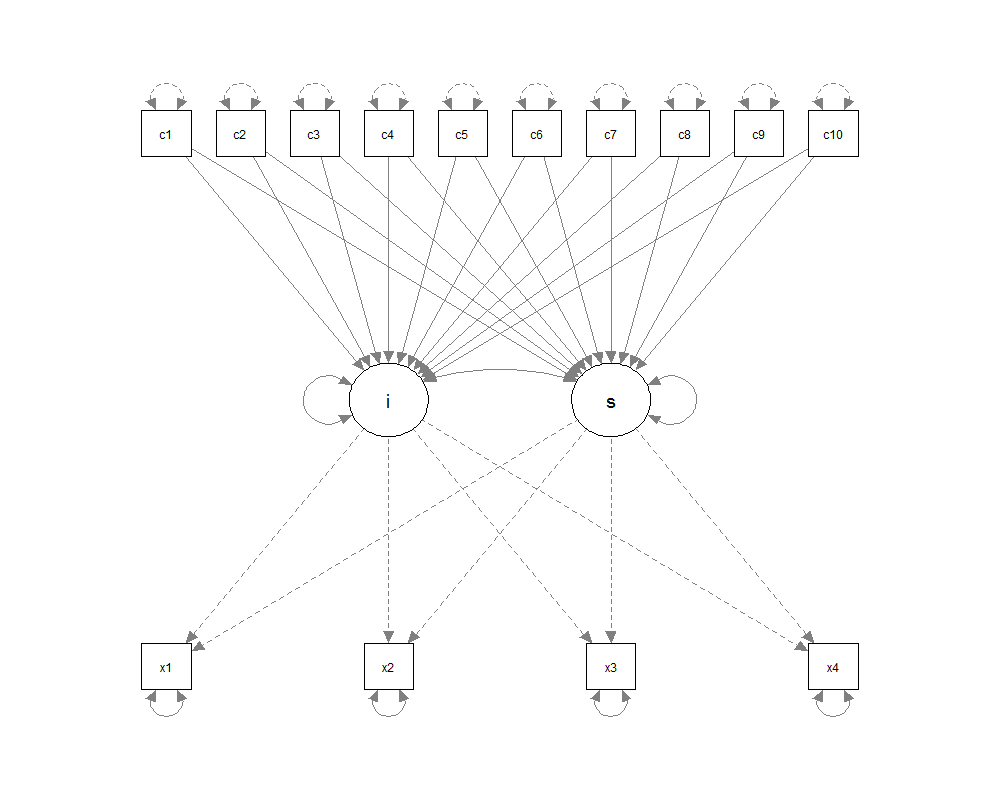
\includegraphics[width=.5\linewidth]{figs/growth_fig}
    \caption{Growth curve model with 10 predictors of both the intercept and slope}
\end{figure}

As an example, a researcher may want to test this model, but may only
have a relatively small sample size (e.g.~80). However, there are 29
estimated parameters in this model, resulting in a estimated parameter
to sample size ratio as far below even the most liberal recommendations
(e.g.~10:1 parameters to sample size; Kline 2015). In lieu of finding
additional respondents, reducing the number of parameters estimated is
one effective strategy. Specifically, the 20 estimated regressions from
\textit{c1-c10} could be reduced to a number that makes the number of
parameters estimated to sample size ratio more reasonable.

\section{Regularization}\label{regularization}

Although a whole host of methods exist to perform variable selection,
the use of regularization has seen a wide array of application in the
context of regression, and more recently, in areas such as graphical
modeling, as well as a host of others. The two most common procedures
for regularization in regression are the \textit{ridge} (Hoerl and
Kennard 1970) and the least absolute shrinkage and selection operator
(\textit{lasso}; Tibshirani 1996); however, there are various
alternative forms that can be seen as subsets or generalizations of
these two procedures. Given an outcome vector \textit{y} and predictor
matrix \(X \in {R}^{n \times p}\) , the ridge estimates are defined as

\[\tag{1}
\hat{\beta}^{ridge}= argmin \Big\{ \sum_{i=1}^{N} (y_{i} = \beta_{0} - \sum_{j=1}^{p}x_{ij} \beta_{j})^{2}  + \lambda \sum_{j=1}^{p} \beta_{j}^{2}\Big\},
\] \noindent
where \(\beta_{0}\) is the intercept, \(\beta_{j}\) is the coefficient
for \(x_{j}\), and \(\lambda\) is the penalty that controls the amount
of shrinkage. Note that when \(\lambda = 0\), equation 3 reduces to
ordinary least squares regression. As \(\lambda\) is increased, the
\(\beta\) parameters are shrunken towards zero. The lasso estimates are
defined as

\[\tag{2}
\hat{\beta}^{lasso}= argmin \Big\{ \sum_{i=1}^{N} (y_{i} = \beta_{0} - \sum_{j=1}^{p}x_{ij} \beta_{j})^{2}  + \lambda \sum_{j=1}^{p}|\beta_{j}|\Big\}.
\]

\noindent
In lasso regression, the \(l_{1}\)-norm is used, instead of
\(l_{2}\)-norm as in ridge, which also shrinks the \(\beta\) parameters,
but additionally drives the parameters all the way to zero, thus
performing a form of subset selection.

In the context of our example depicted in Figure 1, to use lasso
regression to select among the covariates, the growth model would need
to be reduced to two factor scores, which neglects both the relationship
between both the slope and intercept, reducing both to independent
factor scores. Particularly in models with a greater number of latent
variables, this becomes increasing problematic. A method that keeps the
model structure, while allowing for a penalized estimation of specific
parameters is regularized structural equation modeling (RegSEM;
Jacobucci, Grimm, and McArdle 2016). RegSEM adds a penalty function to
the traditional maximum likelihood cost function for SEMs. The maximum
likelihood cost function for SEMs can be written as

\[\tag{3}
F_{ML}=log(\left|\Sigma\right|)+tr(C*\Sigma^{-1})-log(\left|C\right|)- p.
\]

\noindent
where \(\Sigma\) is the model implied covariance matrix, \(C\) is the
observed covariance matrix, and \(p\) is the number of estimated
parameters. RegSem builds in an additional element to penalize certain
model parameters yielding

\[\tag{4}
F_{regsem} = F_{ML} + \lambda P(\cdot)
\]

\noindent
where \(\lambda\) is the regularization parameter and takes on a value
between zero and infinity. When \(\lambda\) is zero, MLE is performed,
and when \(\lambda\) is infinity, all penalized parameters are shrunk to
zero. \(P(\cdot)\) is a general function for summing the values of one
or more of the model's parameter matrices. The two common forms of
\(P(\cdot)\) include both the Lasso (\(\| \cdot \|_{1}\)), which
penalizes the sum of the absolute values of the parameters, and Ridge
(\(\| \cdot \|_{2}\)), which penalizes the sum of the squared values of
the parameters.

In our example, the twenty regression parameters from the covariates to
both the intercept and slope would be penalized. Using lasso penalties,
the absolute value of these twenty parameters would be summed and after
being multiplied by the penalty \(\lambda\), added to equation 4,
resulting in:

\[\tag{5}
F_{lasso} = F_{ML} + \lambda * \left\|  \begin{matrix}  
c1 \xrightarrow[]{} i\\
c2\xrightarrow[]{}i\\
\vdots \\
c10\xrightarrow[]{}i\\
c1\xrightarrow[]{}s\\
\vdots \\
c10\xrightarrow[]{}s\\
\end{matrix}  \right\|_{1}
\]

Although the fit of the model is easily calculated given a set of
parameter estimates, traditional optimization procedures for SEM cannot
be used given the non-differentiable nature of lasso penalties, and as
detailed later, extensions.

\subsection{Optimization}\label{optimization}

One method that has become popular for optimizing penalized likelihood
method is that of proximal gradient descent (e.g.~p.~104 in Hastie,
Tibshirani, and Wainwright 2015). In comparison to one-step procedures
common in SEM optimization, that only involve a method for calculating
the step size and the direction (typically using the gradient and an
approximation of the Hessian), proximal gradient descent can be
formulated as a two-step procedure. With a stepsize of \(\alpha^{t}\)
and parameters \(\theta^{t}\) at iteration \textit{t}:

\begin{enumerate}
    \item First, take a gradient step size $z = \theta^{t} - \alpha^{t} \nabla g(\theta^{t})$.
    \item Second, perform elementwise soft-thresholding $\theta^{t+1} = S_{\alpha^{t} \lambda}(z)$.
\end{enumerate}

where \(S_{\alpha \lambda}(z)\) is the soft-thresholding operator
(Donoho 1995) used to overcome non-differentiability of the lasso
penalty at the origin:

\begin{equation}
S_{\alpha \lambda}(z_{j}) = sign(z_{j})(|z_{j}|-\alpha \lambda)_{+}
\end{equation}

where \((x)_{+}\) is shorthand for max(x,0) and \(\alpha\) is the step
size. Henceforth, \(\lambda\) is assumed to encompass both the penalty
and the step size \(s^{t}\). This procedure is only used to updated
parameters that are subject to penalty. Non-penalized parameters are
updated only using step 1 from above.

In contrast to only updating one parameter at a time in a
coordinate-wise fashion, for RegSEM the optimization steps can be
divided by both the \textit{A} and \textit{S} matrices. This block-wise
gradient descent manifests itself as:

\noindent

\begin{minipage}{\textwidth}
    %   \renewcommand\footnoterule{}    
    \begin{algorithm}[H]
        \begin{algorithmic}[1]
            %   \Procedure{RegSEM Block Coordinate Descent for Lasso}{}
            %   \footnotetext{Note: $A(pen)$ refers only to the penalized parameters, $vec()$ concatenates both vectors}
            \State Generate starting values for $\theta_{t}$
            \State Calculate initial fit $F_{t}$
            \State Set step size $\alpha$. .5 works well at this time.
            \State Set tolerance (tol). e.g. 1e-6
            \While {$|F_{t} - F_{t+1}| > tol$}
            \State Calculate gradient for A:$ \nabla (A) =:  \frac{\partial A}{\partial \theta_{t}}$
            \State $ \theta_{t+1^{*},A} =: \theta_{t,A} - \alpha \nabla(A)$
            \State  Update penalized parameters: $\theta_{t+1^{*},A(pen)} =: S_{\alpha \lambda}(\theta_{t+1^{*},A(pen)})$
            \State Calculate gradient for S:$ \nabla (S) =:  \frac{\partial S}{\partial \theta_{t+1^{*}}}$ 
            \State Update S parameters: $ \theta_{t+1^{*},S} =: \theta_{t,S} - \alpha \nabla(S)$
            \State $\theta_{t+1} =: \theta_{t+1^{*}}$ %vec(\theta_{t+1^{*},A},\theta_{t+1^{*},S})$
            \State Update $S_{t+1}, A_{t+1}$
            \State $ \Sigma_{t+1} = F(I-A_{t+1})^{-1}S_{t+1}(I-A_{t+1})^{-T}F^{T}$
            \State $ F_{t+1} = F_{ML}(\Sigma_{t+1},C) + \lambda \| A_{t+1}(pen) \|$
            \EndWhile
            %   \EndProcedure
        \end{algorithmic}
        \caption{RegSEM Block Coordinate Descent}
        \label{alg:seq}
    \end{algorithm}
\end{minipage}

\noindent
where step 13 is the calculation of the implied covariance matrix using
RAM matrices and step 14 calculates the fit of the model with penalizing
parameters in the \textit{A} matrix. Note that parameters from the
\textit{S} matrix can also be penalized, however, this is much less
common. This algorithm can be described as first order proximal block
coordinate descent. For some SEM models, using block updates has been
found to work better than standard gradient descent with the same soft
thresholding of penalized parameters.

\section{Types of Penalties}\label{types-of-penalties}

Outside of both ridge and lasso penalties, a whole host of additional
forms of regularization exist.

\subsection{Elastic Net}\label{elastic-net}

Most notably, the elastic net (Zou and Hastie 2005) encompasses both the
ridge and lasso, reaching a compromise between both through the addition
of an additional parameter \(\alpha\).

\[
P_{enet}(\theta_{j}) = 0.5(1-\alpha)\| \theta_{j} \|_{2} + \alpha\| \theta_{j} \|_{2}
\]

with a soft-thresholding update of \[
S(\theta_{j})= 
\begin{cases}
0,&  |\theta_{j}| < \alpha\lambda\\
\frac{sgn(\theta_{j})(|\theta_{j}|-\alpha\lambda)}{1+(1-\alpha)\lambda},              & |\theta_{j}|\geq\alpha\lambda
\end{cases}
\]

\noindent
When \(\alpha\) is zero, ridge is performed, and conversely when
\(\alpha\) is 1, lasso regularization is performed. This method
harnesses the benefits of both methods, particularly when variable
selection is warranted (lasso), but there may be collinearity between
the variables (ridge).

\subsection{Adaptive Lasso}\label{adaptive-lasso}

In using lasso penalties, difficulties emerge when the scale of
variables differ dramatically. By only using one value of \(\lambda\),
this can add appreciable bias to the resulting estimates (e.g. Fan and
Li 2001). One method proposed for overcoming this limitation is the
adaptive lasso (Zou 2006). Instead of penalizing parameters directly,
each parameter is scaled by the un-penalized estimated (maximum
likelihood estimate in SEM). This manifests itself as: \[
F_{alasso} = F_{ML} + \lambda \| \theta_{ML}^{-1} * \theta_{pen} \|_{1}
\] \noindent
with, following the same form for the lasso, the soft-thresholding
update is:

\[
S(\theta_{j})= sign(\theta_{j})(|\theta_{j}|-\frac{\lambda}{2|\theta_{j}|})_{+}
\] \noindent
In this, larger penalties are given for non-significant (smaller)
parameters, limiting the bias in estimating larger, significant,
parameters. Note that one limitation of this approach for SEM models is
that the model needs to be estimable with maximum likelihood.
Particularly for models with large numbers of variables, in relation to
sample size, this may not be possible.

\subsection{Smoothly Clipped Absolute Deviation
Penalty}\label{smoothly-clipped-absolute-deviation-penalty}

\begin{figure}
    \centering
    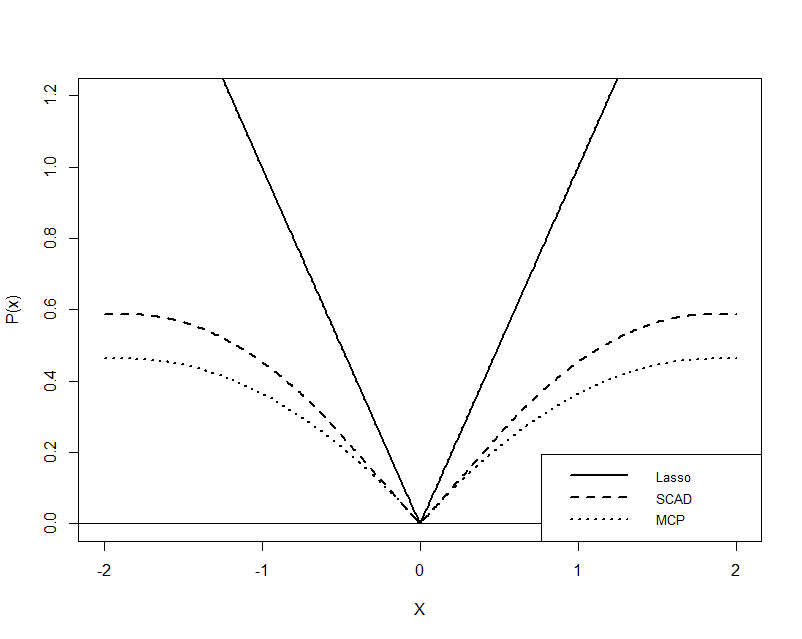
\includegraphics[width=.5\linewidth]{figs/penalties}
    \caption{Comparison of types of penalties with $\lambda=0.5$}
\end{figure}

Two additional penalties that overcome some of the deficiencies of the
lasso, producing sparser solutions, include the smoothly clipped
absolute deviation penalty (SCAD; Fan and Li 2001) and the minimax
concave penalty (MCP; Zhang 2010). In comparison to the lasso, both the
SCAD and MCP have much steeper penalties for smaller parameters, as is
evident in Figure **.

The SCAD takes the form of:

\[
pen_{\lambda,\gamma}(\theta_{j}) = \lambda \big\{I(\theta_{j}\leq\lambda) + \frac{(\gamma \lambda-0)_{+}}{(\gamma-1)\lambda}I(\theta_{j}>\lambda)\big\}
\]

\noindent
with a soft-thresholding update of \[
S(\theta_{j})= 
\begin{cases}
S(\theta_{j},\lambda),&  |\theta_{j}| \geq 2\lambda\\
\frac{\gamma-1}{\gamma-2}S(\theta_{j},\frac{\lambda\gamma}{\gamma-1}),              & 2\lambda < |\theta_{j}|\leq\alpha\lambda\\
\theta_{j} & |\theta_{j}| > \lambda \gamma
\end{cases}
\]

\noindent
As the the penalty in equation 11 is non-convex (as is the MCP), this
makes computation more difficult. However, in the context of SEM this
can be seen as less problematic, as equation 3 is also non-convex.

\subsection{Minimax Concave Penalty}\label{minimax-concave-penalty}

Zhang (2010) proposed the minimax concave penalty:

\[
pen_{\lambda,\gamma}(\theta_{j}) = \lambda\bigg(|\theta_{j}|-\frac{\theta_{j}^{2}}{2\lambda\gamma}\bigg)I(|\theta_{j}|<\lambda\gamma) +\frac{\lambda^{2}\gamma}{2}I(|\theta_{j}|\geq \lambda\gamma)
\]

\noindent
with a soft-thresholding update of \[
S(\theta_{j})= 
\begin{cases}
\frac{\gamma}{\gamma-1}S(\theta_{j},\lambda),&  |\theta_{j}| \leq \lambda\gamma\\
\theta_{j} & |\theta_{j}| > \lambda \gamma
\end{cases}
\]

\noindent
As seen in Figure **, this results in similar amount of shrinkage for
smaller estimates in comparison to the SCAD, however, less for larger
estimates.

\section{Implementation}\label{implementation}

RegSEM is implemented as the \pkg{regsem} package in the \proglang{R}
statistical environment. To estimate the maximum likelihood fit of the
model, \pkg{regsem} uses \textit{Reticular Action Model} (RAM; J. J.
McArdle and McDonald 1984, McArdle (2005)) notation to derive an implied
covariance matrix. The parameters of each SEM are translated into three
matrices: the \textit{filter} (\textit{F}), the \textit{asymmetric}
(\textit{A}; directed paths; e.g.~factor loadings or regressions), and
the \textit{symmetric} (\textit{S}; undirected paths; e.g.~covariances
or variances). See Jacobucci, Grimm, and McArdle (2016) for more detail
on RAM notation.

Syntax for using the \pkg{regsem} is based on the \pkg{lavaan} package
(Rosseel 2012) for structural equation models. \pkg{lavaan} is a general
SEM software program that can fit a wide array of models with various
estimation methods. To use \pkg{regsem}, the user has to first fit the
model in \pkg{lavaan}. As an example, below is the code for a one factor
model fit in lavaan with the Holzinger-Swineford (Holzinger and
Swineford 1939) dataset.

\begin{CodeChunk}
\begin{CodeInput}
library(lavaan)
mod <- "
f1 = ~ NA*x1 + x2 + x3 + x4 + x5 + x6 + x7 + x8 + x9
f1~~1*f1
"
out <- cfa(mod,HolzingerSwineford1939)
\end{CodeInput}
\end{CodeChunk}

After a model is run in lavaan, using \code{lavaan()} or any of the
wrapper functions for fitting a model (i.e. \code{sem()}, \code{cfa()},
or \code{growth()}), the object is then used by the regsem package to
translate the model into RAM notation and run using one of three
functions: \code{regsem()}, \code{multi_optim()}, or \code{cv_regsem}.
The \code{regsem()} function runs a model with one penalty value,
whereas \code{multi_optim()} does the same but allows for the use of
random starting values. However, the main function is \code{cv_regsem()}
as this not only runs the model, but runs it across a vector of varying
penalty values. For instance in the above one-factor model, each of the
factor loadings can be tested with lasso penalties to determine whether
each indicator is a necessary component of the latent factor.

\begin{CodeChunk}
\begin{CodeInput}
library(regsem)
extractMatrices(out)["A"]
out.reg <- cv_regsem(out, type="lasso", 
                    pars_pen=c(1:9),n.lambda=15,jump=.05)
\end{CodeInput}
\end{CodeChunk}

In this, the function \code{extractMatrices()} allows the user to
examine at how the lavaan model is translated into RAM matrices.
Further, by looking at the \textit{A} matrix, the parameter numbers
corresponding to the factor loadings of interest for regularization can
be identified. For this model, the factor loadings represent parameter
numbers one through nine, of which we pass directly to the
\code{pars_pen} argument of the \code{cv_regsem()} function (if
\code{pars_pen=NULL} then all directed effects, outside of intercepts,
are penalized). Additionally, we pass the arguments of how many values
of penalty we want to test (\code{n.lambda=15}), how much the penalty
should increase for each model (\code{jump=.05}), and finally that lasso
estimation is used (\code{type="lasso"}).

The \code{out.reg} object contains two components, \code{out.reg[[1]]}
has the parameter estimates for each of the 15 models, while
\code{out.reg[[2]]} has the fit of each model. For the code above, using
the \pkg{xtable} package to turn the output from \code{out.reg[[2]]}
into a table

\begin{CodeChunk}
\begin{CodeInput}
round(out.reg[[2]],3)
\end{CodeInput}
\begin{CodeOutput}
      lambda conv rmsea      BIC
 [1,]   0.00    0 0.188 7805.177
 [2,]   0.05    0 0.191 7815.389
 [3,]   0.10    0 0.199 7840.590
 [4,]   0.15    0 0.210 7875.842
 [5,]   0.20    0 0.203 7886.147
 [6,]   0.25    0 0.210 7911.816
 [7,]   0.30    0 0.214 7934.454
 [8,]   0.35    0 0.220 7960.670
 [9,]   0.40    0 0.227 7991.033
[10,]   0.45    0 0.229 8009.416
[11,]   0.50    0 0.234 8034.805
[12,]   0.55    0 0.242 8069.487
[13,]   0.60    0 0.286 8360.539
[14,]   0.65    0 0.286 8360.530
[15,]   0.70    0 0.286 8360.525
\end{CodeOutput}
\end{CodeChunk}

In this, the user can examine the penalty (lambda), whether the model
converged (``conv''), with values of 0 indicating convergence, and the
fit of each model. By default, two fit indices are output, both the root
mean square error of approximation (RMSEA; Steiger and Lind 1980), and
the Bayesian information criteria (BIC; Schwarz 1978). Both the RMSEA
and BIC take into account the degrees of freedom of the model, an
important point for model selection in the presence of lasso penalties
(and other penalties that set parameters to zero). This concurs with
work done on degrees of freedom for lasso regression, as Zou, Hastie,
and Tibshirani (2007) proved that the number of nonzero coefficients is
an unbiased estimate of the degrees of freedom for regression. As the
penalty increases, select parameter are set to zero, thus the degrees of
freedom increases, which for fit indices that include the degrees of
freedom in the calculation, means that although the likelihood of the
model may only get worse (increase), both the RMSEA and BIC can improve
(decrease) due to the impact of increased degrees of freedom.

Instead of examining the \code{out.reg[[1]]} output matrix of parameter
estimates, it is easiest to plot the trajectory of each of the penalized
parameters. This is accomplished with \code{plot_cv(out.reg,pars=1:9)},
resulting in:

\begin{CodeChunk}
\begin{CodeInput}
plot_cv(out.reg,pars=1:9)
\end{CodeInput}


\begin{center}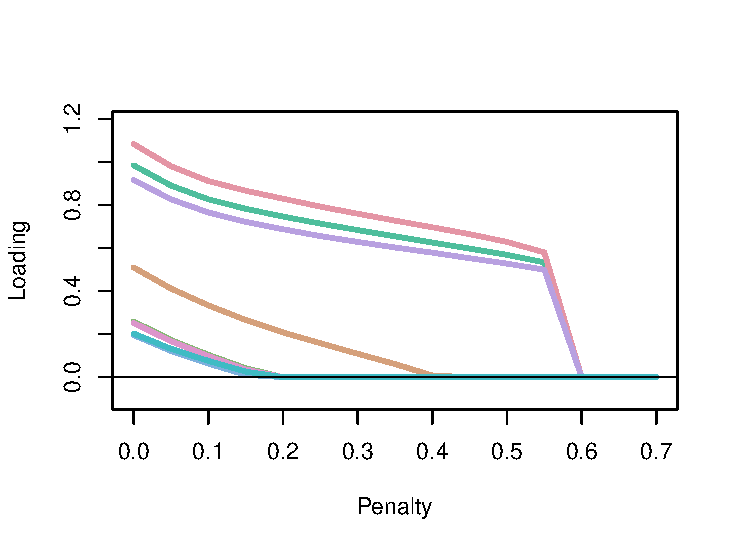
\includegraphics{draft1_files/figure-latex/unnamed-chunk-5-1} \end{center}

\end{CodeChunk}

After a final model (penalty) is chosen, user's have the option either
just use the output from \code{cv_regsem()}, or the final model can be
re-run with either \code{regsem()} or \code{multi_optim()} to attain
additional information. In the model above, the best fitting penalty,
according to the BIC, is \(\lambda=0\). However, for demonstration
purposes, we can choose a penalty of 0.2. With this, the model is re-run
with \code{regsem()}

\begin{CodeChunk}
\begin{CodeInput}
mod.out <- regsem(out, type="lasso", pars_pen=c(1:9),lambda=0.2)
#summary(mod.out)
\end{CodeInput}
\end{CodeChunk}

Note that the arguments used above correspond to the same arguments in
\code{multi_optim()}. However, \code{multi_optim()} has additional
optional arguments corresponding to the number or random starts to try.
Additional fit indices can be attained through the \code{fit_indices()}
function.

\begin{CodeChunk}
\begin{CodeInput}
fit_indices(mod.out)
\end{CodeInput}
\begin{CodeOutput}
$Data_Type
[1] "Train"

$fits
          Fmin         varFit              p          chisq        p.chisq 
       0.69087        0.00000        9.00000      415.90286        0.00000 
          nfac             df           npar              N baseline.chisq 
       1.00000       31.00000       14.00000      301.00000      918.85159 
   baseline.df           logl            ncp          rmsea    rmsea.lower 
      36.00000    -3903.04360        1.28301        0.20344        0.18598 
   rmsea.upper     rmsea.pval            CFI            TLI            BIC 
            NA        0.00000        0.56402        0.49370     7885.98674 
           AIC           CAIC         EBIC.5        EBIC.25 
    7834.08719     7983.11043     8051.12157     8017.06459 
\end{CodeOutput}
\end{CodeChunk}

\noindent
These same fit measures can be accessed through \code{cv_regsem},
through changing the defaults with the \code{fit.ret=c("rmsea","BIC")}
argument. Finally, instead of assessing these fit indices on the same
sample that the models were run on, a holdout dataset could be used.
This can be done two ways: either with
\code{cv_regsem(...,fit.ret2="test")} or with
\code{fit_indices(model,CV=TRUE,CovMat=)} and specifying the name of the
holdout covariance matrix.

\section{Comparison}\label{comparison}

To compare the different types of penalties in \pkg{regsem}, we return
to the the initial example of the latent growth curve model. Using the
same simulated data (see Appendix), the model can be run in \pkg{lavaan}
as

\begin{CodeChunk}
\begin{CodeInput}
mod1 <- "
i =~ 1*x1 + 1*x2 + 1*x3 + 1*x4
s =~ 0*x1 + 1*x2 + 2*x3 + 3*x4
i ~ c1 + c2 + c3 + c4 + c5 + c6 + c7 + c8 + c9 + c10
s ~ c1 + c2 + c3 + c4 + c5 + c6 + c7 + c8 + c9 + c10
"
lav.growth <- growth(mod1,dat,fixed.x=T)
\end{CodeInput}
\end{CodeChunk}

To compare different types of penalties in \pkg{regsem}, it requires a
different specification of the \code{type} argument. The options
currently include maximum likelihood (\code{"none"}), ridge
(\code{"ridge"}), lasso (\code{"lasso"}), adaptive lasso
(\code{"alasso"}), elastic net (\code{"enet"}), SCAD (\code{"scad"}),
and MCP (\code{"mcp"}). For the elastic net, there is an additional
hyperparameter, \(\alpha\) that controls the tradeoff between ridge and
lasso penalties. This is specified as \code{alpha=} , which has a
default of 0.5. Additionally, both the SCAD and MCP have the additional
hyper parameter of \(\gamma\), which is specified as \code{gamma=} and
defaults to 3.7 per Fan and Li (2001).

For the purposes of comparison, each of the 20 covariate regressions
were penalized using the lasso, adaptive lasso, SCAD, and MCP, and
compared to the maximum likelihood estimates (see Appendix for code). In
this model, the data were simulated to have two large effects (both
\textit{c1} parameters), two small effects (both \textit{c2} parameters)
and sixteen true zero effects (\textit{c3-c10} parameters). Note that
the covariates were simulated to have zero covariance among each
variable. If there was substantial collinearity among covariates, the
elastic net would be more appropriate to simultaneously select
predictors while also accounting for the collinearity. The parameter
estimates corresponding the the best fit of the BIC are displayed in
Table *

\begin{table}[ht]
\centering
\begin{tabular}{rrrrrr}
  \hline
 & ML & lasso & alasso & SCAD & MCP \\ 
  \hline
c1 -$>$ i & 0.92* & 0.72 & 0.91 & 0.94 & 0.92 \\ 
  c2 -$>$ i & 0.07 & 0.00 & 0.00 & 0.00 & 0.00 \\ 
  c3 -$>$ i & 0.10 & 0.00 & 0.00 & 0.00 & 0.00 \\ 
  c4 -$>$ i & 0.07 & 0.00 & 0.00 & 0.00 & 0.00 \\ 
  c5 -$>$ i & 0.04 & 0.00 & 0.00 & 0.00 & 0.00 \\ 
  c6 -$>$ i & -0.25 & 0.00 & 0.00 & 0.00 & -0.19 \\ 
  c7 -$>$ i & 0.11 & 0.00 & 0.00 & 0.00 & 0.00 \\ 
  c8 -$>$ i & -0.13 & 0.00 & 0.00 & 0.00 & 0.00 \\ 
  c9 -$>$ i & -0.03 & 0.00 & 0.00 & 0.00 & 0.00 \\ 
  c10 -$>$ i & 0.09 & 0.00 & 0.00 & 0.00 & 0.00 \\ 
  c1 -$>$ s & 1.18* & 1.09 & 1.22 & 1.24 & 1.24 \\ 
  c2 -$>$ s & 0.29* & 0.19 & 0.28 & 0.35 & 0.35 \\ 
  c3 -$>$ s & 0.18 & 0.09 & 0.00 & 0.00 & 0.00 \\ 
  c4 -$>$ s & -0.08 & 0.00 & 0.00 & 0.00 & 0.00 \\ 
  c5 -$>$ s & -0.18 & 0.00 & 0.00 & 0.00 & 0.00 \\ 
  c6 -$>$ s & 0.25* & 0.00 & 0.00 & 0.00 & 0.00 \\ 
  c7 -$>$ s & -0.18 & -0.04 & 0.00 & 0.00 & 0.00 \\ 
  c8 -$>$ s & 0.26* & 0.10 & 0.00 & 0.00 & 0.00 \\ 
  c9 -$>$ s & -0.06 & 0.00 & 0.00 & 0.00 & 0.00 \\ 
  c10 -$>$ s & 0.08 & 0.00 & 0.00 & 0.00 & 0.00 \\ 
  BIC & 3465.28 & 3427.46 & 3415.05 & 3414.38 & 3417.20 \\ 
   \hline
\end{tabular}
\caption{Parameter estimates for the final models across five estimation methods. Note that * represent significant parameters at p < .05 for maximum likelihood estimation.}
\end{table}

While every regularization method erroneously set both simulated true
intercept effects as zero (as in maximum likelihood, which accounts for
these errors), both the adaptive lasso and SCAD correctly identified
every true zero effect. The lasso identified two false effects while the
MCP mistakenly identified one. Additionally, the lasso estimation of the
true effects was attentuated in comparison to the other regularization
methods. This is in line with previous research (cite), necessitating
the use of a two-step relaxed lasso method (Meinshausen 2007, see
Jacobucci, Grimm, and McArdle (2016)) As expected given the small ratio
between number of estimated parameters and sample size, maximum
likelihood mistakenly identified 3 false effects as significant.

To compare the performance of each penalization method further,
particularly in the presence of small number of parameters to sample
size ratios, a small scale simulation study was conducted. The same
model and effects was kept, but the sample size was varied to include
80, 200, and 1000 to demonstrate how maximum likelihood estimation of
effects improves as sample size increases, while each of the
regularization methods performs well regardless of sample size. Each run
was replicated 200 times. The results are displayed in Table *

\begin{table}[ht]
    \centering
    \begin{tabular}{rrrrrrrr}
        \hline
        & N & ML & lasso & alasso & SCAD & MCP \\ 
        \hline
         & 80.00 & 0.09 & 0.05 & \textbf{0.04} & 0.05 & 0.05 \\ 
        False Positives & 200.00 & 0.06 & 0.05 & \textbf{0.02} & 0.03 & 0.04 \\ 
         & 1000.00 & 0.05 & 0.05 & \textbf{0.01} & \textbf{0.01} & 0.19 \\ 
         & 80.00 & 0.45 & \textbf{0.41} & 0.43 & 0.45 & 0.54 \\ 
        False Negatives & 200.00 & 0.30 & \textbf{0.24} & 0.29 & 0.29 & 0.45 \\ 
         & 1000.00 & 0.10 & \textbf{0.09} & 0.17 & 0.19 & 0.24 \\ 
        \hline
    \end{tabular}
    \caption{Results from the simulation using the model in Figure 1. Each condition was replicated 200 times. False positives represent concluding that the simulated regressions of zero were concluded as nonzero. False negatives are concluding that either the simulated regression values of 1 or 0.2 are in fact zero. Bolded values represent the smallest error per condition.}
\end{table}

\section{Discussion}\label{discussion}

This paper provides an introduction to the \pkg{regsem} package,
outlining the mathematical details of the regularized SEM method and the
usage of the package itself.

\subsection{Future Directions}\label{future-directions}

\subsection{Limitations}\label{limitations}

With highly constrained structural equation models, achieving
convergence can be particularly problematic in using \pkg{regsem}. For
instance, with the latent change score model (cite jack), Bayesian
regularization methods have less difficulty in reaching convergence
across chains (cite chapter). With the advent of additional sparsity
inducing priors, along with new forms of software such as STAN (cite
stan), for some models it may be more appropriate to use these Bayesian
regularization methods over their frequentist counterparts.

\subsection*{Conclusion}\label{conclusion}
\addcontentsline{toc}{subsection}{Conclusion}

\hypertarget{refs}{}
\hypertarget{ref-browne2001}{}
Browne, Michael W. 2001. ``An Overview of Analytic Rotation in
Exploratory Factor Analysis.'' \emph{Multivariate Behavioral Research}
36 (1). Taylor \& Francis: 111--50.

\hypertarget{ref-donoho1995noising}{}
Donoho, David L. 1995. ``De-Noising by Soft-Thresholding.'' \emph{IEEE
Transactions on Information Theory} 41 (3). IEEE: 613--27.

\hypertarget{ref-fan2001variable}{}
Fan, Jianqing, and Runze Li. 2001. ``Variable Selection via Nonconcave
Penalized Likelihood and Its Oracle Properties.'' \emph{Journal of the
American Statistical Association} 96 (456). Taylor \& Francis: 1348--60.

\hypertarget{ref-hastie2015statistical}{}
Hastie, Trevor, Robert Tibshirani, and Martin Wainwright. 2015.
\emph{Statistical Learning with Sparsity: The Lasso and
Generalizations}. CRC Press.

\hypertarget{ref-hoerl1970}{}
Hoerl, Arthur E, and Robert W Kennard. 1970. ``Ridge Regression: Biased
Estimation for Nonorthogonal Problems.'' \emph{Technometrics} 12 (1).
Taylor \& Francis Group: 55--67.

\hypertarget{ref-holzinger1939study}{}
Holzinger, Karl John, and Frances Swineford. 1939. ``A Study in Factor
Analysis: The Stability of a Bi-Factor Solution.'' \emph{Supplementary
Educational Monographs}.

\hypertarget{ref-jacobucci2016regularized}{}
Jacobucci, Ross, Kevin J Grimm, and John J McArdle. 2016. ``Regularized
Structural Equation Modeling.'' \emph{Structural Equation Modeling: A
Multidisciplinary Journal} 23 (4). Taylor \& Francis: 555--66.

\hypertarget{ref-kline2015principles}{}
Kline, Rex B. 2015. \emph{Principles and Practice of Structural Equation
Modeling}. Guilford publications.

\hypertarget{ref-lam2009sparsistency}{}
Lam, Clifford, and Jianqing Fan. 2009. ``Sparsistency and Rates of
Convergence in Large Covariance Matrix Estimation.'' \emph{Annals of
Statistics} 37 (6B). NIH Public Access: 4254.

\hypertarget{ref-marsh1996assessing}{}
Marsh, Herbert W, and Kit-Tai Hau. 1996. ``Assessing Goodness of Fit: Is
Parsimony Always Desirable?'' \emph{The Journal of Experimental
Education} 64 (4). Taylor \& Francis: 364--90.

\hypertarget{ref-McArdle_1984}{}
McArdle, J. Jack, and Roderick P. McDonald. 1984. ``Some Algebraic
Properties of the Reticular Action Model for Moment Structures.''
\emph{British Journal of Mathematical and Statistical Psychology} 37
(2). Wiley-Blackwell: 234--51.

\hypertarget{ref-mcardle2005}{}
McArdle, John J. 2005. ``The Development of the Ram Rules for Latent
Variable Structural Equation Modeling.'' \emph{Contemporary
Psychometrics: A Festschrift for Roderick P. McDonald}. Erlbaum. Mahwah,
NJ, 225--73.

\hypertarget{ref-meinshausen2007relaxed}{}
Meinshausen, Nicolai. 2007. ``Relaxed Lasso.'' \emph{Computational
Statistics \& Data Analysis} 52 (1). Elsevier: 374--93.

\hypertarget{ref-raykov1999desirability}{}
Raykov, Tenko, and George A Marcoulides. 1999. ``On Desirability of
Parsimony in Structural Equation Model Selection.'' \emph{Structural
Equation Modeling: A Multidisciplinary Journal} 6 (3). Taylor \&
Francis: 292--300.

\hypertarget{ref-rosseel2012}{}
Rosseel, Yves. 2012. ``Lavaan: An R Package for Structural Equation
Modeling.'' \emph{Journal of Statistical Software} 48 (2): 1--36.

\hypertarget{ref-schwarz1978estimating}{}
Schwarz, Gideon. 1978. ``Estimating the Dimension of a Model.''
\emph{The Annals of Statistics} 6 (2). Institute of Mathematical
Statistics: 461--64.

\hypertarget{ref-steiger1980}{}
Steiger, James H, and John C Lind. 1980. ``Statistically Based Tests for
the Number of Common Factors.'' In \emph{Annual Meeting of the
Psychometric Society, Iowa City, Ia}. Vol. 758.

\hypertarget{ref-thurstone1937}{}
Thurstone, L. L. 1935. \emph{The Vectors of Mind}. Chicago, IL:
University of Chicago Press.

\hypertarget{ref-Tibshirani1996}{}
Tibshirani, Robert. 1996. ``Regression Shrinkage and Selection via the
Lasso.'' \emph{Journal of the Royal Statistical Society. Series B
(Methodological)} 58 (1). Wiley for the Royal Statistical Society:
267--88.

\hypertarget{ref-zhang2010nearly}{}
Zhang, Cun-Hui. 2010. ``Nearly Unbiased Variable Selection Under Minimax
Concave Penalty.'' \emph{The Annals of Statistics} 38 (2). Institute of
Mathematical Statistics: 894--942.

\hypertarget{ref-zou2006adaptive}{}
Zou, Hui. 2006. ``The Adaptive Lasso and Its Oracle Properties.''
\emph{Journal of the American Statistical Association} 101 (476). Taylor
\& Francis: 1418--29.

\hypertarget{ref-zou2005regularization}{}
Zou, Hui, and Trevor Hastie. 2005. ``Regularization and Variable
Selection via the Elastic Net.'' \emph{Journal of the Royal Statistical
Society: Series B (Statistical Methodology)} 67 (2). Wiley Online
Library: 301--20.

\hypertarget{ref-zou2006sparse}{}
Zou, Hui, Trevor Hastie, and Robert Tibshirani. 2006. ``Sparse Principal
Component Analysis.'' \emph{Journal of Computational and Graphical
Statistics} 15 (2). Taylor \& Francis: 265--86.

\hypertarget{ref-Zou2007}{}
---------. 2007. ``On the Degrees of Freedom of the Lasso.'' \emph{The
Annals of Statistics} 35 (5). Institute of Mathematical Statistics:
2173--92.
doi:\href{https://doi.org/10.1214/009053607000000127}{10.1214/009053607000000127}.



\end{document}

